\documentclass[12pt,a4paper]{article}                                                                            
\setlength{\parindent}{2em}          % 首行空两字
\usepackage{fontspec}                % 设置字体
\setmainfont{宋体}
\usepackage{indentfirst}             % 首行缩进

%%%%%%%%%% 数学符号公式 %%%%%%%%%%
\usepackage{xeCJK}                   % 中英文混排
\usepackage{amsmath}                 % AMS LaTeX宏包
%\usepackage{amssymb}                 % 用来排版漂亮的数学公式
%\usepackage{amsbsy}
\usepackage{amsthm}
\usepackage{amsfonts}
\usepackage{mathrsfs}                % 英文花体字体
\usepackage{bm}                      % 数学公式中的黑斜体
\usepackage{bbding,manfnt}           % 一些图标,如 \dbend
\usepackage{lettrine}                % 首字下沉,命令\lettrine
\def\attention{\lettrine[lines=2,lraise=0,nindent=0em]{\large\textdbend\hspace{1mm}}{}}
%\usepackage{relsize}                 % 调整公式字体大小:\mathsmaller,\mathlarger
%\usepackage{caption2}                % 浮动图形和表格标题样式

%%%%%%%%%% 图形支持宏包 %%%%%%%%%%
\usepackage{graphicx}                % 嵌入png图像
\usepackage{color,xcolor}            % 支持彩色文本、底色、文本框等
\usepackage{subfigure}
\usepackage{epsfig}                 % 支持eps图像
%\usepackage{picinpar}               % 图表和文字混排宏包
%\usepackage[verbose]{wrapfig}       % 图表和文字混排宏包
%\usepackage{eso-pic}                % 向文档的部分页加n副图形, 可实现水印效果
%\usepackage{eepic}                  % 扩展的绘图支持
%\usepackage{curves}                 % 绘制复杂曲线
%\usepackage{texdraw}                % 增强的绘图工具
%\usepackage{treedoc}                % 树形图绘制
%\usepackage{pictex}                 % 可以画任意的图形
%\usepackage{hyperref}

%%%%%%%%%%% 列表 %%%%%%%%%%%%%
\usepackage{enumerate}
%\usepackage{algorithm2e}   
\usepackage{algorithm}  
\usepackage{algorithmic}  
\usepackage{float}

%%%%%%%%%% 正文 %%%%%%%%%%
\begin{document}
%%%%%%%%%% 定理类环境的定义 %%%%%%%%%%
%% 必须在导入中文环境之后
\newtheorem{example}{例}             % 整体编号
%\newtheorem{algorithm}{算法}
\newtheorem{theorem}{定理}[section]  % 按 section 编号
\newtheorem{definition}{定义}
\newtheorem{axiom}{公理}
\newtheorem{property}{性质}
\newtheorem{proposition}{命题}
\newtheorem{lemma}{引理}
\newtheorem{corollary}{推论}
\newtheorem{remark}{注解}
\newtheorem{condition}{条件}
\newtheorem{conclusion}{结论}
\newtheorem{assumption}{假设}

%%%%%%%%%% 一些重定义 %%%%%%%%%%
\renewcommand{\contentsname}{目录}     % 将Contents改为目录
\renewcommand{\abstractname}{摘要}     % 将Abstract改为摘要
\renewcommand{\refname}{参考文献}      % 将References改为参考文献
\renewcommand{\indexname}{索引}
\renewcommand{\figurename}{图}
\renewcommand{\tablename}{表}
\renewcommand{\appendixname}{附录}
\renewcommand{\proofname}{证明}
%\renewcommand{\algorithm}{算法}
\renewcommand{\algorithmicrequire}{ \textbf{输入:}} %Use Input in the format of Algorithm  
\renewcommand{\algorithmicensure}{ \textbf{输出:}} %UseOutput in the format of Algorithm  
\renewcommand{\algorithmicrepeat}{ \textbf{循环:}} 
\renewcommand{\algorithmicuntil}{ \textbf{循环停止条件:}} 

%%%%%%%%%% 论文标题、作者等 %%%%%%%%%%
\title{基于p模的协同表达高光谱分类模型}
\author{雷开宇,中国农业大学数学与应用数学系}
%\date{2008年10月01日}                % 日期
\date{2018年4月7日}
\maketitle                            % 生成标题
\tableofcontents                      % 插入目录
\thispagestyle{empty}                 % 首页无页眉页脚

\begin{abstract}
\noindent TODO: 补充摘要,中文摘要300字左右,英文摘要250词左右
\end{abstract}

%\PencilRightUp % 一些可爱的图标,需要bbding宏包的支持
公元1974年,ACM图灵奖授予了Standford大学教授\index{Donald E. Knuth} Donald E. Knuth (高德纳),
表彰他在算法和程序语言设计等多方面杰出的成就。他的巨著 The Art of Computer Programming 令人震撼。
另外,Knuth的突出贡献还包括\index{\TeX 系统} \TeX 系统,毫不夸张地评价,\TeX 给排版带来了一场革命。




%%%%%%%%%% section:选题背景 %%%%%%%%%%
\section{绪论}
\indent   % 恢复缩进

在信息时代....

\subsection{研究背景及意义}
高光谱图像(Hyperspectral Imagery, HSI),是一种通过遥感技术获得的图像。高光谱影像收集及处理整个跨电磁波谱的信息,这些信息是由高光谱传感器(Hyperspectral image sensors)获取并整理。正如人眼一样,人眼能够看到物体,是因为物体反射的光,或者自身发出的光进入眼睛,大脑感受到信号,生成物体影响。与人眼不同的是,人眼只能分辨出可见光,而高光谱图像则可以延伸至红外、紫外,甚至整个电磁波谱上。\\

HSI被广泛应用于农业、地质、天文、化学、食品工程和环境工程等领域,在军事上也有着重要的作用。研究者通过分析HSI来达到不同的目的。例如在地质勘测中,可以通过遥感获取的HSI图像来定位矿区的主要矿种和位置,在环境工程中,通过对有毒气体泄漏区域的空气进行HSI分析,可以确定毒气成分和扩散趋势。

HSI分析中,分类问题是研究的一个热门。在现实中,人们往往能通过专业领域知识来确定出HSI中某个区域的物质构成,以及少量的分布信息。例如在一个利用HSI进行农产品种植结构分析的例子中,人们往往可以通过各地农业部门上报的信息,来确定HSI中存在几种农作物,并且可以根据采样调查知道某个区域农作物的具体分布情况。如何通过这些有限的信息来对整个HSI中的物质进行分类,这是一个值得研究的问题。

机器学习在HSI分类中有着广泛的应用。当人们获取到HSI时,由于人类自身生理结构和极限的限制,直接对HSI进行分析无疑需要大量的人力物力,成本过于高昂。同时,人工方式分类HSI还会受到人类主观心理的影响,例如对图像中特定区域,不同的人可能认为该区域的成分分布不同。随之HSI传感器分辨率越来越高,通过人力直接进行分类变得不再可行,因此使用计算机来对HSI进行分析变得越来越重要。在分类问题中,机器学习能够自主地通过已知信息来学习,因此十分适合HSI分类问题。

从样本数量来说,机器学习分为三类:监督学习、半监督学习和无监督学习。监督学习是将已知标签的样本作为训练集,对样本特征进行学习。无监督学习是指作为训练集的样本没有标签信息,典型的无监督学习有聚类问题。半监督学习是指训练集中既有有标签的样本点,又有无标签的样本点。在本文的假定下,HSI分类问题是一个半监督学习问题,通过数量较少的有标签样本点和部分无标签的样本点构造算法,实现对HSI图像的自动分类。

\subsection{研究现状}
\subsubsection{HSI图像特征}
半监督学习是利用....
\subsubsection{常见的HSI分类问题的解决方案}
\begin{enumerate}
\item 稀疏表达
\item 协同表达
\item SVM
\item 深度学习
\end{enumerate}


\subsection{本文主要工作}
本文主要针对HSI问题的,对协同表达算法进行了改进,使之在HSI分类中表现更好。主要工作有以下几点:
\begin{enumerate}[(1)]
\item 在CR模型的基础上,引入了p模技术,把正则项的中的范数改为p范数,取得更好的稀疏性。
\item 在JCR模型的基础上,引入了p模技术,以得到更好的稀疏性和精确度。
\item 将本文改进后的p-CRC模型、p-JRC模型分别在Indian、Pavia、Salinas等数据集上,与SRC、CRC、JCR和SVM方法进行比较,分析实验结果。
\end{enumerate}

\subsection{本文组织结构}
本文组织结构分为六部分,分别为:绪论、相关知识与理论基础、基于p模的协同表达HSI分类模型、基于p模的联合协同表达HSI分类模型、实验设计与分析、结论与展望。






%%%%%%%%%%% section:相关知识与理论基础 %%%%%%%%%%
\section{相关知识与理论基础}
\subsection{稀疏表达分类模型}
稀疏表示最初是应用在信号处理领域的一种压缩感知方法。稀疏表示的目的是在给定的字典中用尽可能少的元素来表示原信号。但是在近些年,稀疏表示渐渐地与信号处理背景相分离,逐渐成为发展成为了一种称为“字典学习”的机器学习算法。以稀疏表示理论基础的字典学习算法称为“稀疏字典学习(Sparse Representation)”。

设样本集为:
\begin{equation}\label{eq1}
T = \{(x_1, y_1), ... , (x_m, y_l), x_{m + 1}, ... , x_{n + m}\}
\end{equation}
其中,$x_i \in R^d, 1 \leq i \geq m $为输入的数据样本,$m$为已知标签样本点的数量,$n$为未知标签样本点的数量,$y_i, 1 \leq i \geq l$为某个已知标签样本点的标签信息。在稀疏字典学习中,一般将已知标签样本点作为训练集,而将未知标签样本点作为测试集。

对于给定训练集,我们将类别为$l$的已知标签样本集并列到一个矩阵中,组成一个“字典”。记这个字典为$D_{l}$:
\begin{equation}\label{eq2}
D_{l} = [x_1, x2, ... , x_{n_{l}}]
\end{equation}

对于测试集中的样本点$y$,求解以下优化模型:
\begin{equation}\label{eq3}
arg\min_{\alpha} \qquad ||y - D_{l}\alpha||_{2}^{2} + \lambda||\alpha||_{0}
\end{equation}
其中,$\alpha$是线性表达系数,$\lambda||\alpha||_{0}$称为稀疏项,$\lambda$称为稀疏系数。稀疏项使用$l_0$模,该模的定义为:
\begin{equation}\label{eq4}
||x|| = n, \qquad n为x中非零元素的个数
\end{equation}

根据$l_{0}$模的定义,由于稀疏项$\lambda||\alpha||_{0}$的存在,整个优化问题\eqref{eq3}是一个非凸规划。在优化问题中,非凸规划的求解是十分困难的,甚至是无法求解的。值得庆幸的是,人们通过研究发现,在很多情况下,可以通过$l_{1}$模来凸近似$l_{0}$范数,因此稀疏表达的优化问题就变成了:
\begin{equation}
\label{eq5}
arg\min_{\alpha} \quad ||y - D_{l}\alpha||_{2}^{2} + \lambda||\alpha||_{1}
\end{equation}
其中:
\begin{equation}
\label{eq6}
||x||_{1} = \sum_{i = 1}^{n} |x_{i}|, \qquad n为x的维度
\end{equation}

令$r_{l} = ||y - D_{l}\hat{\alpha}||_{2}$,其中$\hat{\alpha}$为优化问题\eqref{eq5}的解,则测试样本$y$类别判断函数为:
\begin{equation*}
label(y) = identity(arg\min_{l}\{r_{l}\})
\end{equation*}

对于\eqref{eq5},我们需要通过迭代的方法来求解近似解。其中,最简单的方法是近端梯度下降法(Proximal Gradient Descent, PGD)。令$\nabla$为微分算子符号,对于优化问题\eqref{eq5}:
$$arg\min_{\alpha} \quad ||y - D_{l}\alpha||_{2}^{2} + \lambda||\alpha||_{1}$$
令$f(x) = ||y - D_{l}\alpha||_{2}^{2}$,显然,$f(x)$可微且$\nabla f(x)$满足如下的$Lipschitz$条件:

\begin{definition}
$\exists \beta > 0$, 使得$\forall x_{1}, x_{2}$\\
\begin{equation*}
||\nabla f(x_{1}) - \nabla f(x_{2})|| < \beta ||x_{1} - x_{2}||
\end{equation*}
\end{definition}

因此,在定义域上某点$x_{k}$附近,$f(x)$可通过展开为二阶泰勒公式:
\begin{equation}
\label{eq7}
\hat{f}(x) \simeq f(x_{k}) + \nabla f(x_{k})^{T}(x - x_{k}) + o(||x - x_{k}||_{2}^{2})
\end{equation}

由上述$Lipschitz$条件可以得出,$\exists L > 0$,使得:
\begin{equation*}
\frac{||\nabla f(x_{1}) - \nabla f(x_{2})||_{2}^{2}}{||x_{1} - x_{2}||_{2}^{2}} < L
\end{equation*}
则\eqref{eq7}就等价于:
\begin{align}
\hat{f}(x) & \simeq f(x_{k}) + \nabla f(x_{k})^{T}(x - x_{k}) + \frac{L}{2}||x - x_{k}||_{2}^{2} \label{eq8}\\
	& = \frac{L}{2}||x - (x_{k} - \frac{1}{L} \nabla f(x_{k}))||_{2}^{2} + const \label{eq9}
\end{align}
其中$const$是与$x$无关的常数。可以看出,使用梯度下降法对原函数$f(x)$进行最小化,实际上就等价于对$\hat{f}(x)$进行最小化,即对式\eqref{eq9}进行最小化。式\eqref{eq9}的最小值可通过求导解出,其最小值在$x_{k + 1}$处获得:
\begin{equation*}
x_{k + 1} = x_{k} - \frac{1}{L} \nabla f(x_{k})
\end{equation*}

将上述思路带回优化问题\eqref{eq5}中,可得$PGD$的每一步迭代应为:
\begin{equation}
\label{eq10}
\alpha_{k + 1} = arg\min_{\alpha} \frac{L}{2}||\alpha - (\alpha_{k} - \frac{1}{L} \nabla f(\alpha_{k}))||_{2}^{2} + \lambda ||\alpha||_{1}
\end{equation}


稀疏表达的本质,其实是利用尽可能少的资源,来表示尽可能多的知识。这样可以带来的附加好处,就是会缓解存储压力。事实上,在“字典学习”中,当样本的数量级十分巨大时,字典学习的任务还包括对字典$D$进行学习,通过特征选择去除一些与学习任务无关的特征。这种情况下算法更为复杂,常见的算法有$K-SVD$算法。在HSI分类问题中,相比样本数量,样本的维度较小,因此使用\eqref{eq5}所表示的优化问题即可。


\subsection{协同表达分类模型}
协同表达分类模型与稀疏表达分类模型思路相似,均为通过字典来表示测试点。不同于稀疏表达,协同表达分类模型中,使用的是$l_{2}$正则化,而不是$l_{1}$正则化。

协同表达中,对前述的$T, D_{l}, y$,求解优化问题:
\begin{equation}
\label{eq11}
arg\min_{\alpha} \qquad ||y - D_{l}\alpha||_{2}^{2} + \lambda||\alpha||_{2}^{2}
\end{equation}
令$\hat{\alpha}$为优化问题\eqref{eq11}的最优解,记$r_{l}$为测试点$y$与其近似线性表达的残差:
\begin{equation*}
r_{l} = \frac{||y - D_{l}\hat{\alpha}||_{2}}{||\hat{\alpha}||_{2}}
\end{equation*}
测试样本点$y$的判别函数为:
\begin{equation*}
label(y) = identity(arg\min_{l}\{r_{l}\})
\end{equation*}

不同于SRC,CRC的求解过程是十分简单的。由于$l_{2}$范数具有可微性,因此优化问题\eqref{eq11}存在解析解:
\begin{equation}
\label{eq12}
\hat{\alpha} = (D_{l}^{T}D_{l} + \lambda I)^{-1}D_{l}^{T}y
\end{equation}

以下是协同表达分类模型的算法:

\begin{algorithm}[H] 
	\caption{Collabortative Representation Classifier}  
	\label{alg:CRC}  
	\begin{algorithmic}
		\REQUIRE 
			测试样本点$y$,训练样本集${D_{l}}$,参数$\lambda$;
		\ENSURE 
			样本类别$identity(y)$;
		\STATE $\quad$
		\STATE {令$l = 1$}   
		\REPEAT   
			\STATE 选取$D_{l}$,计算$U = (D_{l}^{T}D_{l} + \lambda I)^{-1}D_{l}^{T}$ 
			\STATE 计算$\hat{\alpha} = Uy$
			\STATE 计算$r_{l} = \frac{||y - D_{l}\hat{\alpha}||_{2}}{||\hat{\alpha}||_{2}}$
		\UNTIL {训练样本全部计算完毕\\}  
		\STATE 计算$identiy(y) = arg\max_{l} \{r_{l}\}$
	\end{algorithmic}  
\end{algorithm}  

文献\cite{Zhang L}中,Zhang Lei将SRC与CRC进行了对比,结果表明,在人脸识别领域,CRC能够达到与SRC相近的分类效果,甚至在面对面部有遮挡的情况也有着较为优秀的效果。在HSI分类领域,CRC也取得了较为成功的应用。众多研究者们通过不断对CRC进行改进,使之在HSI分类问题中有了很好的表现。



%%%%%%%%%%% section:基于$l_{p}$范数的协同表达HSI分类模型 %%%%%%%%%%
\section{基于$l_{p}$范数的协同表达HSI分类模型}
\subsection{岭回归与$l_{p}$范数}
我们首先考虑一个回归问题。假设对训练集$A = \{(x_{1}, y_{1}), ... , (x_{m}, y_{m})\}$进行最小二回归,其中$x_{i} \in \mathbb{R}_{d}, y_{i} \in \mathbb{R}, 1 \leq i \leq m$。

我们知道,最小二乘发进行回归时,要求解如下的二次优化问题:
\begin{equation}
\label{eq13}
\min_{w} \sum_{i = 1}^{m} (y_{i} - w^{T}x_{i})^2
\end{equation}

我们知道,最小二乘法很容易陷入“过拟合”的状态,即过度关注了模型在训练集上的误差,导致模型在训练集上的误差很小,而在测试集上的误差很大的情况。过拟合一般发生在\textbf{样本点(相对样本特征)不足}的情况。在机器学习中,人们往往希望通过增加训练集来解决过拟合问题,但是在很多场景中无法做到这点。为了在不增加训练集的情况下解决过拟合,研究者引入了多种正则化项。这些正则化项中,最常见的正则化项是$l_{2}$正则项,即在优化问题\eqref{eq13}目标函数中增加$w$的$l_{2}$范数:
\begin{equation}
\label{eq14}
\min_{w} \sum_{i = 1}^{m} (y_{i} - w^{T}w_{i})^2 + \lambda||w||_{2}^{2}
\end{equation}

其中,参数$\lambda$ 称为正则化参数,一般$\lambda > 0$。优化问题\eqref{14}被称为“\textbf{岭回归(Ridge Regression)}”,由Tikhonov与Arsenin在1977年提出。

在$l_{2}$正则项的基础上,人们将其推广为$l_{p}$正则项,即使用$l_{p}$范数进行正则化,解决过拟合现象。数学中,$l_{p}$范数被定义为:
\begin{equation*}
||x||_{p} = \sqrt[p]{\sum_{i}^{n} x_{i}^{p}}
\end{equation*}
优化问题\eqref{eq14}就变成了:
\begin{equation}
\label{eq15}
\min_{w} \sum_{i = 1}^{m} (y_{i} - w^{T}w_{i})^2 + \lambda||w||_{p}^{p}
\end{equation}
由以上定义可得,稀疏表达中稀疏项所使用的$l_{1}$范数、协同表达中的正则项使用的$l_{2}$也属于$l_{p}$范数。当使用$l_{1}$范数时,优化问题\eqref{eq15}称为LASSO(Least Absolute Shrinkage and Selection Operator)回归,由Tibshirani于1996年提出。

相比$l_{2}$范数,使用$l_{p}$范数更易得到“稀疏解”,其直观表示如下图所示

\begin{figure}[H] 
\center
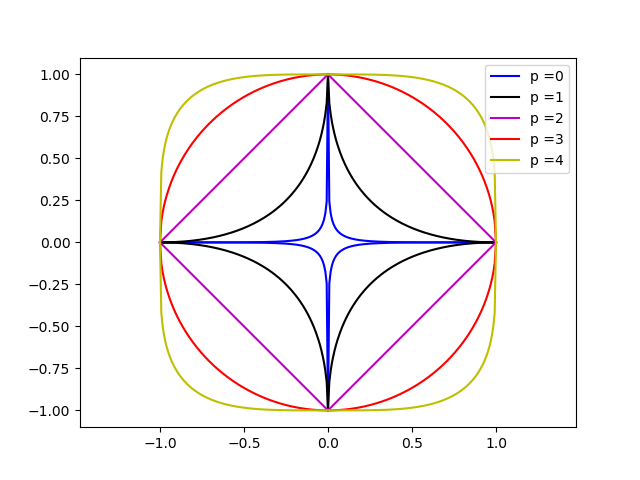
\includegraphics[width=3.5in]{lp_norm.png} 
\caption{$l_{p}$范数}\label{fig:1} 
\end{figure} 

显然,当$p$在0到2之间时,$l_{p}$范数能够计算出出较为优异的稀疏解。


\subsection{Tikhonov矩阵}

\subsection{降维方法}
在数据挖掘与机器学习中,由高维空间引起的维数灾难常常是令人头痛的。维度灾难会使得计算复杂度呈指数型向上升,因此,在高维度数据挖掘中,进行特征提取,降低原数据的维度成为了必要的步骤。

\begin{definition}
对样本集合$X = \{x_{}, ..., x_{N}\} \in R^{m \times N}, x_{i} \in R^{m}$,降维问题指的是:建立一个$R^{m} \longmapsto R^{d}, m > d$的一个映射矩阵$A \in R^{m \times d}$,使得原样本通过映射$z_{i} = A^{T}x_{i}$对应到低维子空间$R^{d}$上的点。
\end{definition}

通过降维操作,我们能够显著地减小模型的计算复杂度。除此之外,降维还可以剔除原样本中的冗余信息,凸显出对数据影响最大的一些特征。

一般来讲,降维分为特征选择和特征提取两种,前者是在原有特征(后者称为属性)中选择出一些主要特征,而后者则是将原特征进行综合考虑,形成一些新的特征。在HSI中,每个像素背后都对应着一条光谱带,通常为220维,我们要确定某类物质,往往并不需要对全部的220个特征进行判断,因此我们可以通过降维来减少计算量,以加快运算速度。

在我们的模型中,我们主要使用主成分分析(PCA)方法与线性判别法(LDA)来降维。

\subsubsection{主成分分析PCA}
主成分分析(Principal components analysis)是最常用的一种特征提取方法,其主要思想在于从数据的原始空间中提取主要特征,即主成分,降低样本维度,同时尽可能保持原始空间中数据的相对位置。

设有二维样本集$X = \{x_{1}, ... , x_{N}\}, x_{i} \in R^{2}$,我们希望通过PCA将该样本集降维到一维空间,即一条直线上。如下图所示,
\begin{figure}[H] 
% \center
% 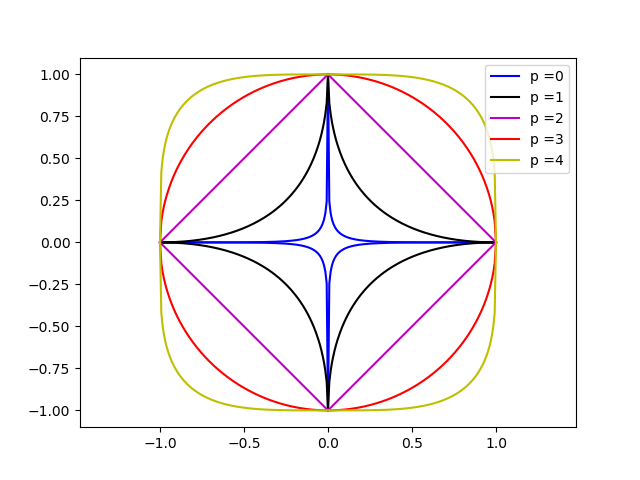
\includegraphics[width=3.5in]{lp_norm.png} 
% \caption{$l_{p}$范数}
\label{fig:2} 
\end{figure} 
我们想要寻找的这条直线应该满足这样的条件:
\begin{enumerate}[(1)]
\item 最近重构性:样本点$x_{1}, ... , x_{n}$到直线的距离应该尽可能小;
\item 最大可分性:样本点$x_{i}, ... , x_{n}$在直线上的投影应该尽可能散落。
\end{enumerate}
设样本点$x_{i}$在直线上的投影为$z_{i}$,则满足条件(1)的直线可通过如下优化问题来求解:
\begin{equation}
\label{eq16}
\min \sum_{i = 1}^{N}||x_{i} - z_{i}||^{2}
\end{equation}
设直线的单位方向向量为$w = {a, b}$,则$z_{i}$可以表示为:$z_{i} = w^{T}x_{i}$。

为了使直线满足条件(2),我们需要构建优化问题:
\begin{equation}
\label{eq17}
\max \sum_{i = 1}^{N}||z_{i} - \bar{z}||^{2}
\end{equation}
其中$\bar{z}$是$z_{i}$的平均值,即$\bar{z} = \frac{1}{N}\sum_{i = 1}^{N}z_{i}$。

通过线性代数的推导,我们可以发现,优化问题\eqref{eq16}与\eqref{eq17}的目标函数其实是等价的,二者都可以转变成:
\begin{equation}
\label{eq18}
\max tr(w S w)
\end{equation}
其中,$S = \sum_{i = i}^{N}(x_{i} - \bar{x})(x_{i} - \bar{x})^{T}$,$\bar{x}$表示$x_{i}$的平均值。$S$为原样本的协方差矩阵,用来表示原样本的整体离散度。

优化问题\eqref{eq17}可以直接推广到高维空间,且易知$S = XX^{T}$。设$X = {x_{1}, ... , x_{N}}, x_{i} \in R^{m  \times N}$ 我们可以在高维空间上构造出同样的优化问题:
\begin{equation}
\label{eq19}
\begin{split}
arg\min_{W} & \quad tr(W^{T}XX^{T}W) \\
s.t. & \quad W^{T}W = I
\end{split}
\end{equation}
其中,$W = {w_{i}, ... , w_{m}}$为投影变换后的坐标系且$w_{i}$为该坐标系的标准正交基向量。计算优化问题\eqref{eq19},得到新的坐标系$W$。

根据线性空间理论和拉格朗日乘方法,优化问题\eqref{eq19}等价于:
\begin{equation}
\label{eq20}
arg \min_{W} tr(W^{T}XX^{T}W - \Lambda (W^{T}W - I))
\end{equation}
其中$\Lambda = {\lambda_{1}, ... , \lambda_{d}}$为拉格朗日系数。

优化问题\eqref{eq20}可直接通过求导来得到其极值:

令$F(W) = W^{T}XX^{T}W - \lambda (W^{T}W - I)$,
当$F(W)$的导数$dF(W)$为零时,有
\begin{align*}
0 &= dF(W)\\
  &= 2XX^{T}W - 2\Lambda W\\
  &= XX^{T}W - \Lambda W  
\end{align*}
即:
\begin{equation}
\label{eq21}
XX^{T}w_{i} = \lambda_{i} w_{i}
\end{equation}
显然,满足\eqref{eq21}的$lambda_{i}, w_{i}$实质为矩阵$XX^{T}$的特征值与特征向量。因此优化问题\eqref{eq19}就转变成了对协方差矩阵$S$进行特征值分解,我们将特征值按照从小到大的顺序重新排列为${\lambda_{1}, ... , \lambda_{d}}$,按照特征值的顺序排列特征向量,得到的
\begin{equation*}
W = {w_{1}, ... , w_{d}}
\end{equation*}
即为\eqref{eq19}的解,原样本的映射为$z_{i} = W^{T}x_{i}$。


这样得到的新的坐标系同原样本空间的维度是相同的,为了达成降维的目的,还需要舍去$W$中的部分坐标。通常降维后的空间维度$d^{'}$是根据重构阈值$t$来确定:
\begin{equation}
\label{eq22}
\frac{\sum_{i = 1}^{d^{'}} \lambda_{i}}{\sum_{i = 1}^{d} \lambda_{i}} \geq t
\end{equation}
最终的$d^{'}$就是使上式成立的最小的$d^{'}$。

主成分分析降维算法如下:
\begin{algorithm}[H] 
	\caption{主成分分析:Principal components analysis}  
	\label{alg:PCA}  
	\begin{algorithmic}
		\REQUIRE 
			原样本$X = \{x_{i}\}$;
		\STATE \textbf{步骤:}
		\STATE 1. 中心化样本:$x_{i} := x_{i} - \frac{1}{m}\sum_{i = 1}^{m}x_{i}$;   
		\STATE 2. 计算协方差矩阵$S = XX^{T}$;
		\STATE 3. 对$S$进行特征值分解,并将特征值从大到小进行排列;
		\STATE 4. 根据公式\eqref{eq22}确定$d^{'}$;
		\STATE 5. 计算前$d^{'}$个特征值的特征向量$w_{i}$,输出投影矩阵$P = \{w_{1}, ... , w_{d^{'}}\}$;
		\STATE 6. 计算降维后的投影$z_{i} = P^{T}x_{i}$。
	\end{algorithmic}  
\end{algorithm}  

\subsubsection{线性判别分析LDA}
线性判别分析

\subsection{基于$l_p$范数的协同表达分类模型(pCRC)}

\subsubsection{pCRC-1}
正如前文所述,相比$l_{2}$范数,$l_{p}$范数能够增加模型的稀疏性,得到更好的学习表现,同时减少内存存储压力;相比$l_{1}$范数,$l_{p}$范数一定程度上又能加速训练速度,因此,我们不妨考虑使用$l_{p}$范数作为协同表达的正则项。

对比优化问题\eqref{eq5}与\eqref{eq11},我们可以对比二者得到的表达系数$\alpha$。图\eqref{fig:3}表示的是在测试点$y$与训练集$X$在同样参数$\lambda$下的测试结果。
\begin{figure}[H] 
\center
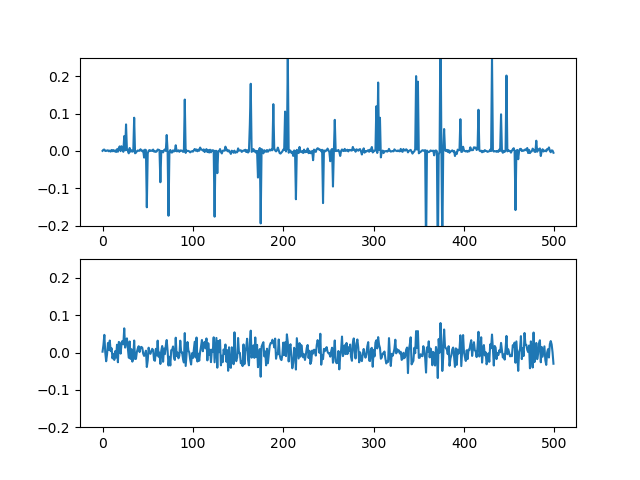
\includegraphics[width=4in]{l2_vs_l1.png} 
\caption{$l_{1}$范数与$l_{2}$范数对比}
\label{fig:3} 
\end{figure}
其中,上图表示的是$l_{1}$范数得到的$\alpha$,下图表示的是$l_{2}$范数下得到的$\alpha$。显然,$l_{1}$范数得到的结果更加稀疏。在字典学习中,稀疏的表达系数往往能够体现出与测试样本相关性比较大的训练样本。根据线性空间理论,如果一个样本处于某个线性子空间中,该样本可以表示成该子空间一组极大线性无关组的线性组合。假设高光谱数据中,每一类样本处于同一线性子空间中,那么



%%%%%%%%%%% section:实验与分析 %%%%%%%%%%
\section{实验与分析}
这个\TeX 模板只是为了提供一个学习\TeX 的参考,各节的内容并没有关联性。欢迎读者使用并改进该模板,
并祝学习\TeX 愉快!

Knuth大师最初设计\TeX 的时候并没有想到中文化,\TeX 排版系统的中文化始终令初学者望而却步、云山雾罩。
类UNIX系统下的teTeX和Windows系统下的MikTeX,都是\TeX 知名的发行版。然而,teTeX已经停止研发五年之久,
基于MikTeX的中文发行版CTeX 虽然如火如荼,但依然挡不住\TeX Live 一统江湖的大趋势。

虽然\TeX Live 还未入住FreeBSD的ports tree,但teTeX的远去,
令FreeBSD之下的很多ports不得不面临改换门庭的窘境。例如,auctex、latex-cjk等等。


\TeX 的中文化可以有多种途径,xelatex 是其中最简单的(不见得是最美观的)。
在\TeX Live 2011 之下,不需要有任何更多的设置,甚至不用考虑中英文混排,
xelatex能满足绝大多数中文化要求。这对于初学者来说,无疑是一个福音。


%%%%%%%%%% 参考文献 %%%%%%%%%%
\begin{thebibliography}{}
\bibitem[1]{Zhang L} Zhang L, Yang M, Feng X. Sparse representation or collaborative representation: Which helps face recognition?[C]//Computer vision (ICCV), 2011 IEEE international conference on. IEEE, 2011: 471-478.
\bibitem[2]{Wei Li}Li W, Du Q. Joint within-class collaborative representation for hyperspectral image classification[J]. IEEE Journal of Selected Topics in Applied Earth Observations and Remote Sensing, 2014, 7(6): 2200-2208.
\end{thebibliography}
\clearpage
\end{document}
%%%%%%%%%% 结束 %%%%%%%%%%